\documentclass{zpt}
\title{实验三: SLR分析器}
\begin{document}
    \maketitle
    \tableofcontents
    \clearpage
    \section{实验内容}
    用C++实现对给定文法的SLR语法分析器。
    \section{程序设计原理与方法}
    \subsection{原理}
    使用\textbf{SLR分析器}
    \begin{itemize}
        \item 对输入字符串进行词法分析, 将其解析为句子
        \item 根据给定文法求各个符号的$\mathsf{First},\mathsf{Follow}$集
        \item 根据给定文法创建一系列项目
        \item 求项目的闭包$\mathsf{Closure}$以及转移函数$\mathsf{Go}$
        \item 构造SLR分析表
        \item 进行LR分析
    \end{itemize}
    \subsection{方法}
    明确了原理后, 参照课本, 进行一步步实现。不得不说, SLR分析器比LL(1)难写太多了;\par
    和上一个实验一样, 我使用\textbf{类}来实现, 目的有三个:\begin{enumerate}
        \item \textbf{最少化所需的对应关系表的数量}。 比如用map存某个symbol对应的first集这种, 统统不需要;
        \item \textbf{最大化程序的灵活程度}。 由于所有操作对象都是指针, 我们可以轻松地完成对元素的访问, 比如通过文法类访问其左端的符号, 再比如通过项目类访问对应的文法, 通过闭包访问其中某个项目的某个文法的某个右端符号的序号等;
        \item \textbf{最小化占用的空间};
        \item \textbf{更好地抽象出符号, 文法, 闭包, 分析器的概念}, 方便自己的理解, 以及后续能够方便地引入到别的文件中;
    \end{enumerate}
    具体来说, 我分别定义了如下8个类:
    \begin{lstlisting}[language=c++]
// 符号类
class Symbol{
    public:
        char symbol;                        // 具体符号
        int index;                          // 符号的序号, 对应在最终的分析表中的行号/列号
        bool is_terminal;                   // 是否是终结符

        Symbol();
        Symbol(char,int,bool);

        set<Symbol*> first;                 // First集
        set<Symbol*> follow;                // Follow集

        int append_first(Symbol*,int);
        int append_follow(Symbol*, int);

        void printFirst();
        void printFollow();
};

// 符号集
class Symbols{
    public:
        Symbols();
        void info();                        // 打印符号集中所有符号的相关信息

        void append(Symbol*);               // 给符号集添加新的符号
        Symbol* find(char);                 // 根据符号的值查找某一个符号

        set<Symbol*> symbols;               // 用集合保存符号集中符号的指针

        int length;                         // 符号个数
};

// 文法类
class Grammer{
    public:
        Grammer();
        Symbol* head;                       // 文法的左式, 直接对应到相应的符号
        vector<Symbol*> tail;               // 文法的右式, 用vector按顺序保存右端的所有符号

        void info();                        // 输出文法信息
};

// 项目类
class Item{
    public:
        Item();
        Item(Grammer*, int, int);

        Symbol* get_dot();                  // 获取.之后的那个符号的指针
        Symbol* get_head();                 // 获取项目头符号的指针

        void info();

        Grammer* grammer;                   // 保存该项目对应的文法的指针
        Item* next;                         // 保存下一个项目的指针

        int dot;                            // .的位置
        int index;                          // 项目序号
        int length;                         // 项目长度(对应文法的右部的长度)
};

// 项目集类(闭包类)
class Items{
    public:
        Items();
        Items(int);

        Items* find_route(char);            // 根据路由表查询某一个字符在DFA上对应的下一个闭包

        bool append(Item *, bool=false);    // 往项目集中添加新项目
        void info();
        vector<Item*> items;                // 用动态数组保存项目
        set<int> indices;                   // 维护一个项目的id的集合, 用来判断某两个项目集是否相等
        map<char, Items*> route;            // 路由表
        int index;                          // 闭包序号(状态号)
};

// 闭包集类
class Closures{
    public:
        Closures();
        Closures(int);
        vector<Items*> closures;            //用动态数组保存闭包的指针

        Items* find(Items*);                // 在数组中查询某一个闭包
        void get_closure_and_go(map<char, vector<Items*>>&, map<char, Symbol*>&);               // 计算所有闭包和对应的go函数
        void info();

        int length;                         // 闭包的个数
};

// 文法集类
class Grammers{
    public:
        Grammers();
        Grammers(int);                          // 创建给定个数的新文法
        int len();                              // 有效的文法长度
        void info();

        Grammer& operator[](int);               // 重载[]使得该操作符能够直接访问其grammer成员
        vector<Items*>& operator[](char);       // 重载[]使得能直接访问其items成员

        void get_grammer(ifstream&, map<char, Symbol*>&, Symbols&);   // 读入并加载文法, 为所有独特的符号创建一个实例

        vector<Grammer*> grammers;              // 用动态数组保存文法
        map<char, vector<Items*>> items;        // 用map保存某一个符号开头的项目集的数组

        int length;
};

// 分析器类
class Parser{
    public:
        Parser(Grammers&,Symbols&,Symbols&,Symbols&);   // 构造函数, 将各个成员赋值
        void get_symbols();                              // 根据读取的文法, 创建两个符号集, 对应终结符和非终结符
        void initialize(const string&);                 // 进行一系列初始化操作, 包括构建符号集, 加载文法, 计算闭包等
        void get_first();                                // 计算每一个符号的first集
        void get_follow();                               // 计算每一个符号的follow集
        void get_table();                                // 根据闭包和Go, 构建分析表
        void parse(string,string);                      // 从给定输入文件读取输入并分词, 然后写入给定输出文件中, 之后进行语法分析
        void error();                                   // 出错的响应函数

        Grammer *** action;                             // action表, 表的单元是语法类的指针
        int ** goTo;                                    // goto表, 表的单元是状态序号
    private:
        Grammers grammers;
        map<char, Symbol*> symbols;                     // 总的单词表
        Symbols terminals;
        Symbols nterminals;

        Closures closures;                              // 所有闭包

        int get_lex(vector<deque<Symbol*>>&, string&, string&);  // 进行词法分析的函数
        int _id(char);
};
    \end{lstlisting}

    \section{程序设计流程}
    根据上一个section, 在完善了各个类的定义后, 我需要说明一下代码的逻辑:\begin{itemize}
        \item 文法集类实例parser.grammers调用grammers.get\_grammer读取老师给的文法, 在此函数中完成两件事:\begin{itemize}
            \item 为所有symbol创建实例, 将指针保存在分析器实例的属性parser.symbols中
            \item 为所有文法构建对应的项目实例, 注意\textbf{项目实例不需要保存文法的头尾, 只需要保留一个文法的指针, 然后用一个int来指明.的位置即可}。 之后, 从同一个文法中构建的项目形成一个\textbf{项目集}, 进一步, 以同一个非终结符开头的所有项目集被保存在一个vector中, 存在文法集实例的属性items中。由于是按顺序保存各个项目, 所以每个项目集的第一个都是.XX, 这有助于我们之后构建闭包;
        \end{itemize}
        \item 分析器调用parser.get\_symbol将parser.symbols中的符号划分为terminals和nterminals, 然后调用parser.get\_first, parser.get\_follow分别计算每个符号的first集和follow集;
        \item 闭包集类实例parser.closures调用closures.get\_closure\_and\_go计算closure集和go函数, 这里主要采用两个方法:\begin{itemize}
            \item 通过\textbf{维护一个set}来求某一个item的闭包;
            \item 通过\textbf{广度优先搜索}来计算所有go函数;
        \end{itemize}
        \item 分析器调用parser.get\_table构建action表和goto表;
        \item 分析器调用parser.parse()进行分析。
    \end{itemize}
    由上, 整个语法分析的流程被极大地简化, 我在主程序中只需要实例化分析器, 然后调用两个分析器的方法即可完成语法分析。值得一提的是, 由于使用了私有变量保存符号类等, 类外是无法干扰编译程序运行的。
    \begin{figure}[H]
        \centering
        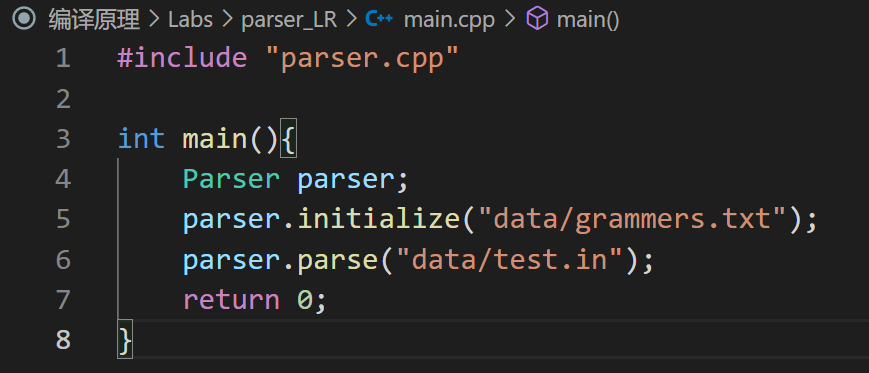
\includegraphics[width=\textwidth]{../resources/main.png}
    \end{figure}

    \subsection{和词法分析器的串联}
    需要注意的是, 实验中让设计的语法分析器是对给定的四则运算的, 那个$\mathbf{id}$根据我的理解就代表着\emph{identifier}, 也就是任何\textbf{整数, 小数, 变量};而将输入的字符串解析为有意义的符号集, 即句型, 是靠词法分析器的, 因此我将实验一的词法分析器整合到实验二中, 对每一个输入字符串, 都是\textbf{先词法分析, 再读取中间文件, 然后语法分析。}\par
    这里不得不说, 老师给的文法还是相当简单的, 如果要完成整个c--的文法, 其实应该会更复杂。\par
    除此之外, 我的分析器支持\textbf{多行分析}。


    \section{程序设计清单}
    如上, 我们要设计实现八个类, 其相应的成员函数, 同时要把词法分析器的内容做一些修改, 同时, 实验一我图懒省事, 所有代码放在一个.cpp文件中, 而且lexer也不是一个类, 使用函数封装的, 在整合时我就感受到了很多不方便之处, 这也是我在parser使用类的一个重要原因。\par
    更多地, 在本实验中, 我将代码组织为经典的.h声明, .cpp定义的结构, 最后在main.cpp中运行, 很优雅。\par

    \section{运行结果}
    将多个运算表达式写入test.in, 其中包含数字, 小数和identifier, 进行语法分析, 得到结果部分展示如\reff{fig::input}$\sim$\reff{fig::sentence1}:
    \begin{figure}
        \centering
        \begin{subfigure}[t]{0.45\textwidth}
            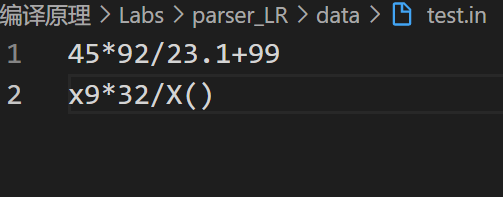
\includegraphics[width=\textwidth]{../resources/input.png}
            \caption{input}
            \label{fig::input}
        \end{subfigure}
        \begin{subfigure}[t]{0.45\textwidth}
            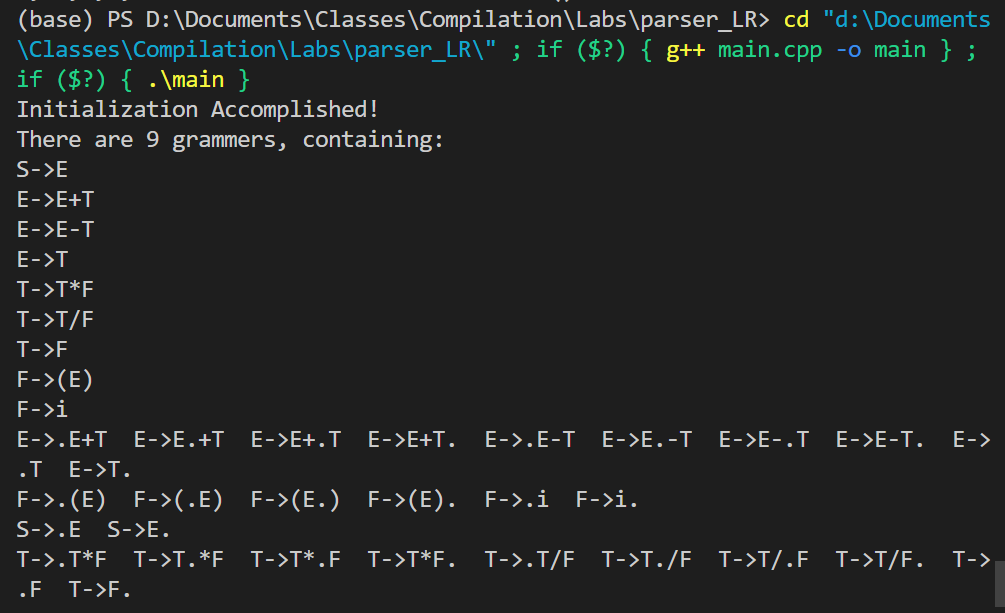
\includegraphics[width=\textwidth]{../resources/grammers.png}
            \caption{grammers and items}
            \label{fig::grammer}
        \end{subfigure}
        \begin{subfigure}[t]{0.45\textwidth}
            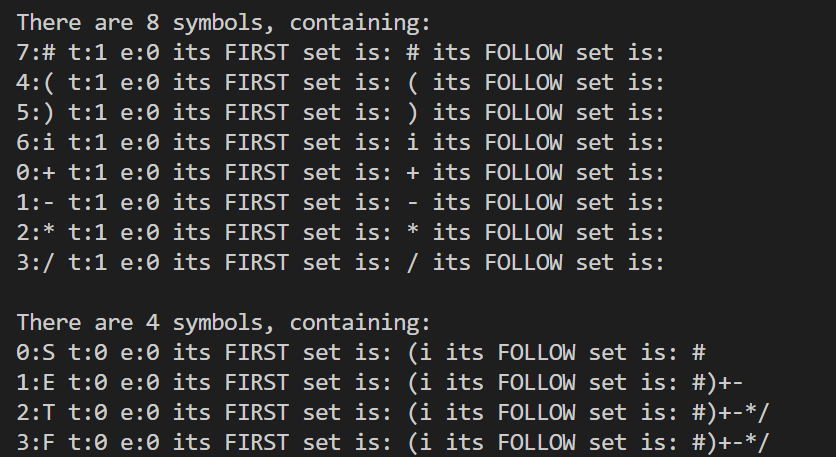
\includegraphics[width=\textwidth]{../resources/symbols.png}
            \caption{symbols}
            \label{fig::symbol}
        \end{subfigure}
        \begin{subfigure}[t]{0.45\textwidth}
            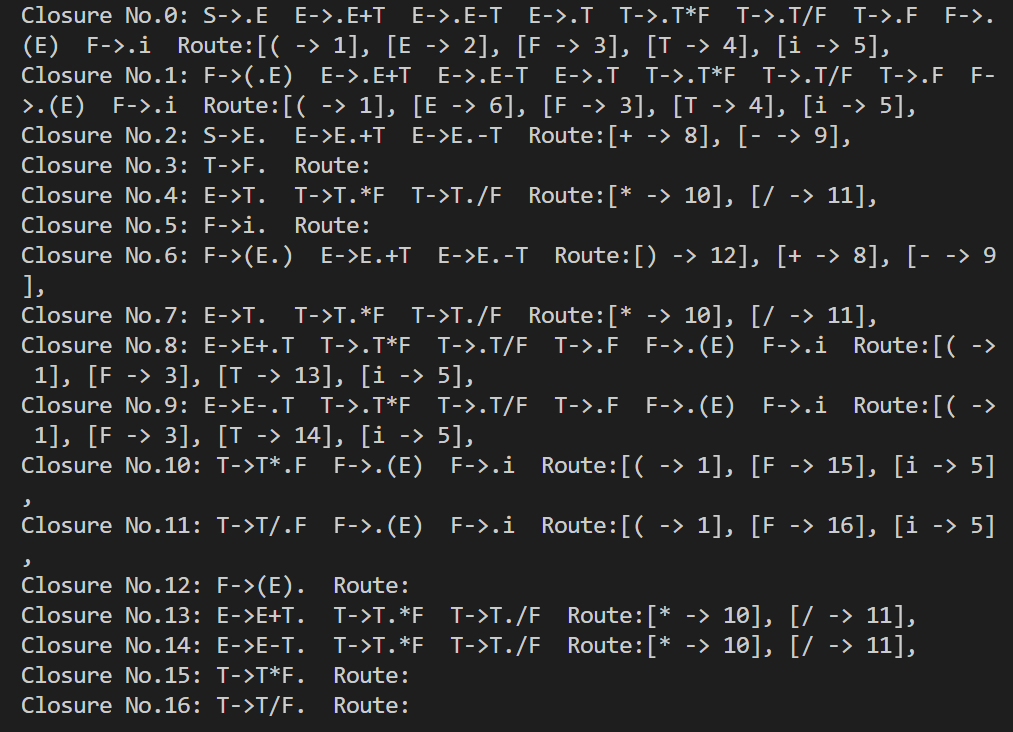
\includegraphics[width=\textwidth]{../resources/closures.png}
            \caption{closures}
            \label{fig::closure}
        \end{subfigure}
        \begin{subfigure}[t]{0.45\textwidth}
            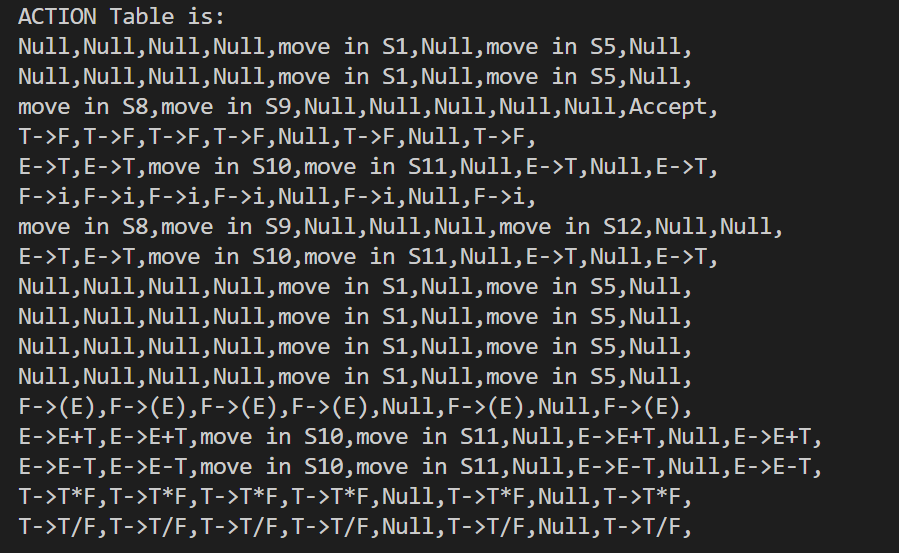
\includegraphics[width=\textwidth]{../resources/action.png}
            \caption{action table}
            \label{fig::action}
        \end{subfigure}
        \begin{subfigure}[t]{0.45\textwidth}
            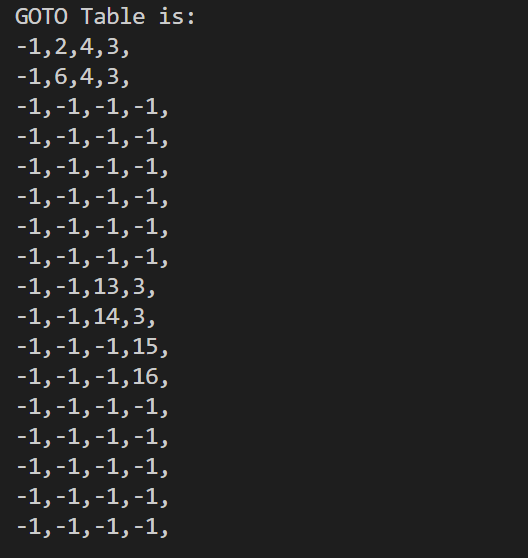
\includegraphics[width=\textwidth]{../resources/goto.png}
            \caption{closures}
            \label{fig::goto}
        \end{subfigure}
        \begin{subfigure}[t]{0.45\textwidth}
            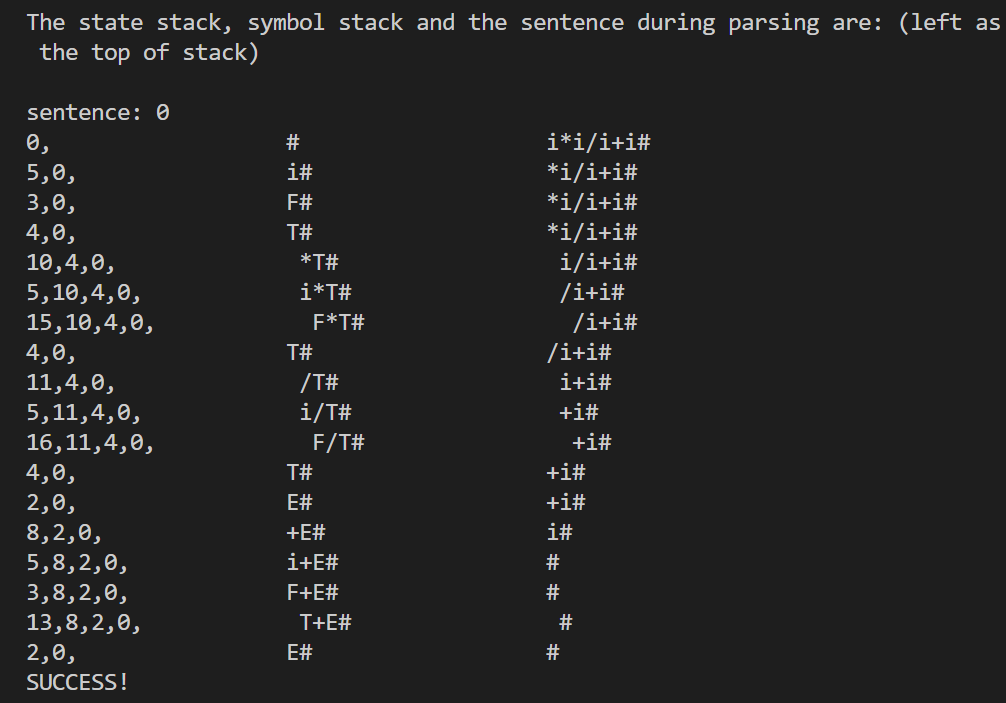
\includegraphics[width=\textwidth]{../resources/output1.png}
            \caption{result for the first sentence}
            \label{fig::output1}
        \end{subfigure}
        \begin{subfigure}[t]{0.45\textwidth}
            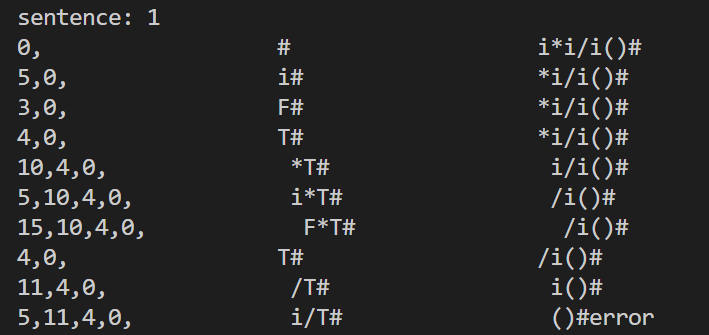
\includegraphics[width=\textwidth]{../resources/output2.png}
            \caption{result for the second sentence}
            \label{fig::output2}
        \end{subfigure}
        \caption{运行结果}
    \end{figure}
    \section{程序使用说明}
    \begin{itemize}
        \item 在data/test.in中修改要解析的字符串;
        \item 在data/grammers.txt中修改给定的文法;
        \item 在data/KeyWords.txt中修改预设关键词;
        \item 在data/Operators.txt中修改预设操作符;
        \item 在data/Separators.txt中修改预设分隔符;
        \item 语法分析的结果默认会在终端显示;
    \end{itemize}
    \section{总结与完善}
    通过这次实验, 回忆了c++的类写法, 从头到尾搞明白了SLR的分析逻辑, 自己完成了各项算法的设计;同时也遗留了几个问题:
    \begin{itemize}
        \item 在求$\mathsf{Closure}$时应该可以更快, 而且感觉我一直不是很擅长写\emph{“到不增大为止”}这种条件的代码。
    \end{itemize}
\end{document}